\documentclass[a4paper,12pt]{article}
\usepackage{listing}
\usepackage{graphicx}
\begin{document}


    \title{13. Simple Mail Transfer Protocol}
    \author{Santhisenan A}
    \date{\today}
    \maketitle

\section{Aim}
Implement Simple Mail Transfer Protocol

\section { Simple Mail Transfer Protocol}
Email is emerging as the one of the most valuable service in internet today. 
Most of the internet systems use SMTP as a method to transfer mail from one user to another. 
SMTP is a push protocol and is used to send the mail whereas POP (post office protocol) 
or IMAP (internet message access protocol) are used to retrieve those mails at the receiver’s side.

\subsection{SMTP Fundamentals}
SMTP is an application layer protocol. The client who wants to send the mail opens a TCP connection to the 
SMTP server and then sends the mail across the connection. The SMTP server is always on listening mode. 
As soon as it listens for a TCP connection from any client, the SMTP process initiates a connection on that port 
(25). After successfully establishing the TCP connection the client process sends the mail instantly.

\section{SMTP Protocol}
SMTP uses commands and responses to transfer messages between an MTA client and an
 MTA server. The command is from an MTA client to an MTA server; the response is 
 from an MTA server to the MTA client. Each command or reply is terminated by a 
 two- character (carriage return and line feed) end-of-line token.
 
 \subsection{Commands}
 Commands are sent from the client to the server.
 It consists of a keyword followed by zero or more arguments.

 \subsection{Responses}
 Responses are sent from the server to the client. A response is a 
 three- digit code that may be followed by additional textual information.

\begin{figure}
	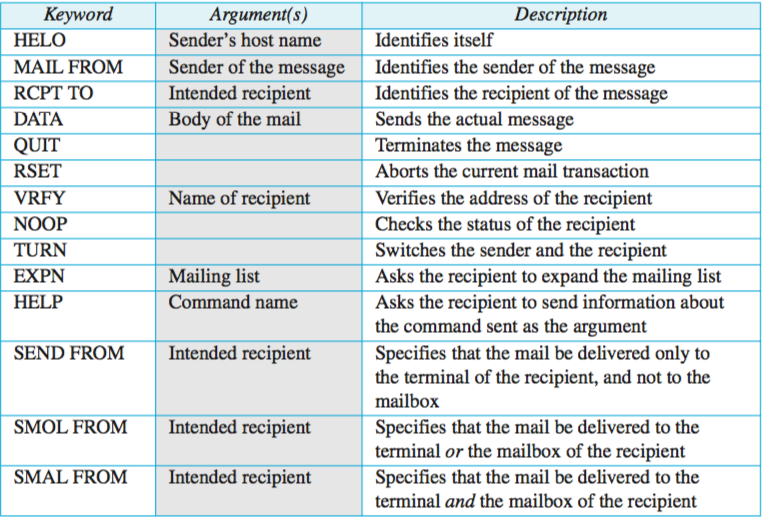
\includegraphics[width=\linewidth]{./SMTPcommads.png}
	\caption{SMTP Commands}
	\label{fig:smtpcommands}
\end{figure}
\begin{figure}
	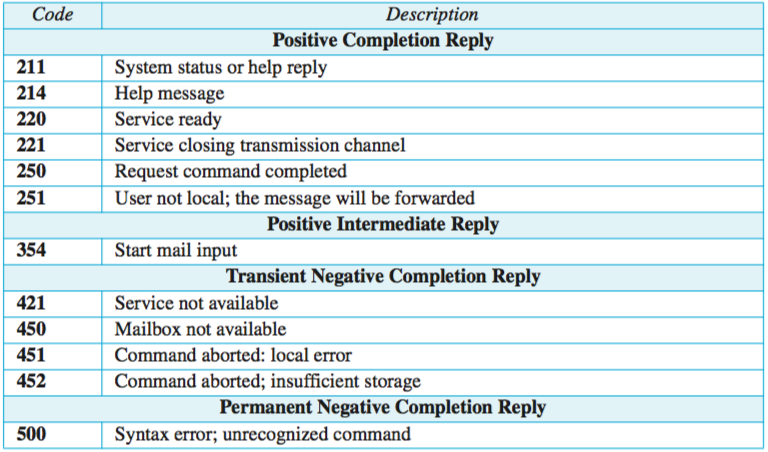
\includegraphics[width=\linewidth]{./SMTPresponses.png}
	\caption{SMTP Responses}
	\label{fig:smtpcommands}
\end{figure}
\begin{figure}
	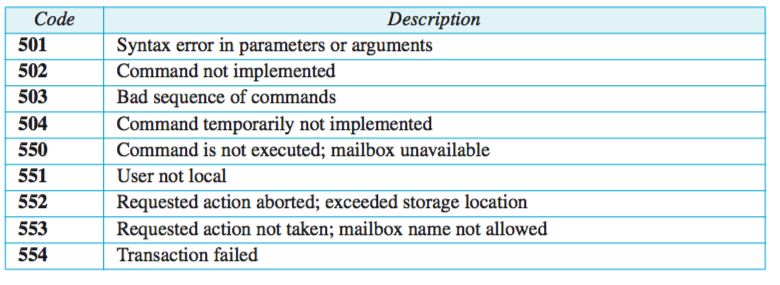
\includegraphics[width=\linewidth]{./SMTPresponses1.png}
	\caption{SMTP Responses (contd.)}
	\label{fig:smtpcommands}
\end{figure}

\pagebreak

% \subsection{Model of SMTP system}



% In the SMTP model user deals with the user agent (UA) for example Microsoft outlook, netscape, Mozilla etc. 
% In order to exchange the mail using TCP, MTA is used. The users sending the mail do not have to deal with the 
% MTA it is the responsibility of the system admin to set up the local MTA. The MTA maintains a small queue of mails
% so that it can schedule repeat delivery of mail in case the receiver is not available. The MTA delivers the mail
% to the mailboxes and the information can later be downloaded by the user agents.

% Both the SMTP-client and MSTP-server should have 2 components:
% \begin{itemize}
% \item User agent (UA)
% \item Local MTA  
% \end{itemize}


% Communication between sender and the receiver :
% \begin{itemize}
% \item The senders, user agent prepare the message and send it to the MTA . 

% \item The MTA functioning is to transfer the mail across the network to the receivers MTA.
  
% \end{itemize}


% \subsection{Sending Email}

% Mail is send by a series of request and response messages between the client and a server. 
% The message which is send across consists of a header and the body. A null line is used to terminate the mail
%  header. Everything which is after the null line is considered as body of the message which is a sequence of ASCII
%   characters.The message body contains the actual information read by the receipt.

% \subsection{Receiving Email}

% The user agent at the server side checks the mailboxes at a particular time of intervals. 
% If any information is received it informs the user about the mail. When user tries to read the mail it displays a 
% list of mails with a short description of each mail in the mailbox. By selecting any of the mail user can view
% its contents on the terminal.
\section{Mail Transfer Phases}
\subsection{Connection Establishment}
After a client has made a TCP connection to port 25, the server starts the connection 
phase.
This phase includes 3 phases:
\begin{itemize}
    \item The server sends code 220 (Service Ready) to tell the client that it is ready 
    to recieve the mail. If the server is not ready, it sends 421 (service unavailable).
    \item The client sends HELO message to identify itself using its domain name and
    address. This step informs the server of the domain name of the client.
    \item The server responds with a code 250 (Request Command Completed) or some other 
    code depending on the situation.
\end{itemize}

\subsection{Message Transfer}
After connection has been established between the SMTP client and server, 
a single message between a sender and one or more recipients can be exchanged. 
This phase involves eight steps. Steps 3 and 4 are repeated if there is more than 
one recipient.

\begin{itemize}
    \item The client sends the MAIL FROM message to introduce the sender of the 
    message. It includes the mail address of the sender (mailbox and the domain 
    name). This step is needed to give the server the return mail address for 
    returning errors and reporting messages.

    \item The server responds with code 250 or some other appropriate code.

    \item The client sends the RCPT TO (recipient) message, which includes the mail address
    of the recipient.

    \item The server responds with code 250 or some other appropriate code.

    \item The client sends the DATA message to initialize the message transfer.

    \item The server responds with code 354 (start mail input) or some other appropriate
    message.

    \item The client sends the contents of the message in consecutive lines. 
    Each line is ter- minated by a two-character end-of-line token 
    (carriage return and line feed). The message is terminated by a line 
    containing just one period.

    \item The server responds with code 250 (OK) or some other appropriate code.

\end{itemize}

\subsection{Connection Termination}
After the message is transferred successfully, the client ter- minates the connection. 
This phase involves two steps.
\begin{itemize}
    \item The client sends the QUIT command.
    \item The server responds with code 221 or some other appropriate code.
\end{itemize}

\section{Code}

\section{Output}

\end{document}